% Snippet from paper draft (Gradient-Landscape Diagnostic + Fig.~3).
% Image file in this directory: bp_main_3x2.pdf
\subsection{Gradient-Landscape Diagnostic}\label{sec:bp}

We conduct a barren-plateau diagnostic \cite{BarrenPlateauOriginal,Ragone2024,Fontana2024} for all three injection variants. At each grid point, we draw $K=256$ independent PQC initialisations $\theta_q^{(k)}\sim p_0(\theta_q)$ from the same Gaussian prior used during training, freeze all classical parameters, and measure the per-parameter loss gradient $\partial\mathcal{L}/\partial\theta_q^{(k)}$ on a single fixed mini-batch from each benchmark. Gradients are computed with the same TorchDEQ IFT backward used in \S\ref{sec:experiments}, so the reported variance matches the optimisation signal seen at the start of training. We sweep the qubit count $n_q\in\{2,4,6,8,10\}$ at fixed $R=1$, and the circuit repetition count $R\in\{1,2,3,4,6,8\}$ at fixed $n_q=4$, while keeping the solver budget fixed at $T=50$. 

Each grid point is subject to a wall-clock budget of $2400\,\mathrm{s}$. When the IFT backward does not finish all $K$ resamples within this budget (this occurs for SD and BD at $n_q=10$ on PROTEINS in our runs), we still report the variance estimated from the completed samples, but mark the point with an open symbol annotated by the completed/requested count in Fig.~\ref{fig:bp-main}; such points are excluded from the log-linear fit. Additional implementation details are provided in Appendix~\ref{app:repro}.


Figure~\ref{fig:bp-main} shows a pronounced absolute-magnitude separation between IN and the two dependent variants. Along the qubit-count sweep, the gradient-variance ratio between IN and SD at the largest evaluated point is $10^{3.09}$ on NCI1 ($n_q=10$), $10^{4.52}$ on PROTEINS ($n_q=8$, the largest qubit count for which SD completes within budget), and $10^{3.16}$ on MUTAG ($n_q=10$). Along the depth sweep, the corresponding IN-to-SD ratio is $10^{1.84}$ on NCI1 ($R=8$) and $10^{3.18}$ on MUTAG ($R=8$). Over all finite grid points, IN exceeds both dependent variants at $30$ of $32$ locations in Fig.~\ref{fig:bp-main}; the two exceptions both occur on the PROTEINS depth sweep and are discussed below.\footnote{On PROTEINS at $R=1$ and $R=8$, IN yields variances of $7.5\times 10^{-9}$ and $9.4\times 10^{-6}$, below SD's $3.7\times 10^{-5}$ and $1.4\times 10^{-5}$, respectively. Inspection of the per-initialisation loss on this batch suggests that, at $R=1$, IN and BD produce outputs near the classifier origin (mean cross-entropy $0.58$), whereas SD produces outputs much farther from it (mean cross-entropy $10.4$), and the gradient magnitudes follow the same ordering. We report these cases as observed, without adjustment.}

Across all panels, the fitted log-linear slopes of $\log_{10}\mathrm{Var}_{\theta_q}[\cdot]$ remain small in magnitude ($|s|\le 0.32$), and are mostly positive over the range $(n_q\le 10,\; R\le 8)$ considered here. By contrast, the dominant pattern in Fig.~\ref{fig:bp-main} is the absolute-magnitude separation between IN and the dependent variants: under the same training-time backward pass, IN typically produces gradient variances that are three to four orders of magnitude larger than those of SD and BD along the qubit-count sweep.

\begin{figure}[t]
    \centering
    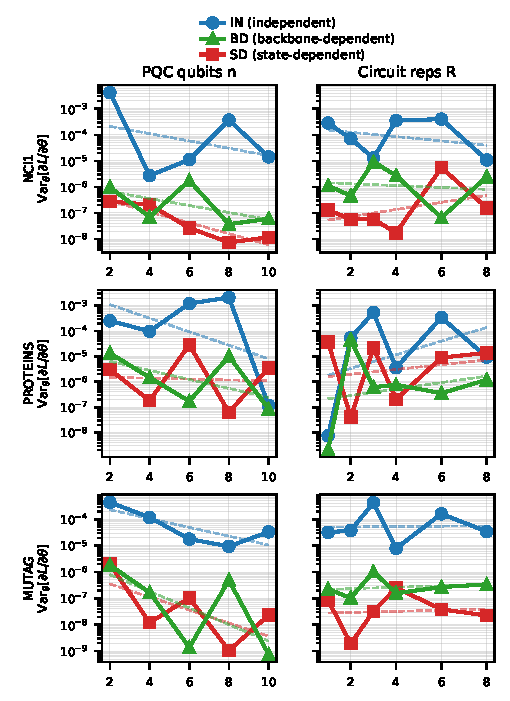
\includegraphics[width=\columnwidth]{bp_main_3x2.pdf}
    \caption{PQC gradient variance at random initialisation on NCI1, PROTEINS, and MUTAG, computed with the TorchDEQ IFT backward used during training. Rows correspond to datasets. Left column: qubit-count sweep $n_q\in\{2,4,6,8,10\}$ with $R=1$. Right column: repetition sweep $R\in\{1,2,3,4,6,8\}$ with $n_q=4$. Each point aggregates $K=256$ random PQC initialisations, and the reported quantity is $\mathrm{Var}_{\theta_q}[\partial\mathcal{L}/\partial\theta_q]$ averaged over PQC parameters. Dashed lines show log-linear fits. Open markers indicate grid points where the per-point wall-clock budget was reached before all $K$ resamples completed; the completed/requested ratio is shown next to each such point, and these points are excluded from the fit.}
    \label{fig:bp-main}
\end{figure}

Taken together, these results support the IN-versus-dependent ordering suggested in Remark~\ref{rem:ordering}, which is the main design-level comparison of this paper. By contrast, we do not claim a reliable empirical separation between BD and SD from this diagnostic alone: across the scanned grid, the two dependent variants remain close, and the random-initialisation variance of a single gradient component is not sufficiently discriminative in this regime.
